% !TeX root = ../main.tex
% Add the above to each chapter to make compiling the PDF easier in some editors.
\chapter{Design}\label{chapter:analysis}

\begin{comment}
\section{Overall Design}
Our architecture comprises the following:
\begin{enumerate}
	\item An Android Application
	\item A server application
	\item A public database (with a visualizing website)
\end{enumerate}

\subsection{Android Application}
The Android Application needs the following:
\begin{enumerate}
	\item \textcolor{green}{Create a public/private key pair}
	\item \textcolor{green}{Automatically collect Location Raw Data for the scheme {Timestamp, Location} --> TODO: Implement database in Android Application}
	\item Ensure that even when the app is not running, data is collected.
	\item Create activities from the location raw data for the scheme {From, To, Duration, type, ...}
	\item Algorithm to infer home and work location (or ask for home / work location (rough specification)).
	\item For each day? week?, ... compute the areas where the user was active. (This can be done as an aggregation request as well)
	\item Stage 2: (or even stage 1?): After each day, send anonymously, thus over several nodes, in which area the device has been active! \sout{(that is a breach of our privacy!!! find solution) in order for the server to know to whom send requests regarding locations.} \textcolor{red}{The most possible fine level of user location will be stored alongsied the id}
	\item Send registration request to server application (including most coarse location). If successful, less coarse location will be send until unscuccessful. The server will store the request for the least coarse location area and count the following requests. Once a threshold is met, it will "unlock" this location.
	\item Mobile might send (privacy?!?!?!) most coarse location after one week etc. again. TODO: Think about least coarse area useful. (city, department, ... level)
	The location can be more coarse than needed for the aggregation request. This will create network overhead, thus a balance has to be found.
	\item receive Aggregation request from server application
	\item calculate response to aggregation request
	\item Apply logic when to abort aggregation request e.g when incoming n is 0 and next device ID is empty.
	\item send aggregation response
	\item At least one screen displaying some text / information about the application and hinting to turn off battery saving mode
	\item Automatic hard-coded push notification to check for an update at date xxx
	\item Automatic hard-coded deletion of all data after test-phase including a push notification to ask for the deinstallation of the app.
\end{enumerate}
In stage two, the App will also be able to send e.g. traffic alerts to the server.

\subsection{Server application}
The server application needs the following:
\begin{enumerate}
	\item A database containing counters for each level of reported active location to "unlock them".
	\item A database listing all registered devices following the scheme {public device key, Google Cloud messaging key (for reaching the device), most accurate possible last location}.
	\item A database containing all possible aggregation requests
	\item A scheduler to start / send out aggregation requests
	\item A handler for an ongoing aggregation request (forward it to the next one, until done or aborted).
	\item Store a requests result in the public database
\end{enumerate}
In stage 2, the server also processes data send by the client on its own behalf.
The server aggregation task does the following
\begin{itemize}
	\item \sout{Randomly select a fake-start-n (out of the range of lets say 1-5) in order } \textcolor{red}{With encryption not necessary}
	\item \sout{Select fake-start-value} \textcolor{red}{Not necessary with encryption}
	\item Devices list for the aggregation request (Will be made dynamic in stage 2).
\end{itemize}

\subsection{Public database}
The public database comprises the following schemes for aggregation requests.
Furthermore, it handles incoming data e.g. traffic alerts.
The aggregation schemes will all contain at least the following fields:
\begin{itemize}
	\item Current n
	\item Current mean / value \textbf{Use json (or xml) for value passing}
	\item ID ?? (necessary?)
	\item Next device's public key for encryption of the data (and n?)
	\item Timestamp start
	\item Tmestamp end --> duration
\end{itemize}
\end{comment}
\section{Specific designs}
\subsection{Standard user story}
Our user is called Hans
\begin{enumerate}
	\item Hans somehow gets motivated to go to the playstore and install our appliation
	\item In the playstore, Hans sees some photos and information about the application
	\item Hans clicks on the install button in the playstore to install our application. The installation process starts.
	\item Hans is curious about the application and opens the application.
	\item Hans sees the first and only screen of the application that tells hime what the application does. It also contains a link to view the results stored in the public database.
	\item (In stage 2, maybe Hans can even see his data and what has been send, ...)
	\item Hans leaves the application (the application must still go on in the background).
	\item Hans uses his task manager to quit the application (the application must still go on collecting data in the background).
	\item After some days, without Hans being involved, an aggregation request is started and send to the appliation running in the background.
	\item The application receives and processes the request and sends the results to the server without Hans noticing anything.
	\item One week after the installation, tha application creates a push notification and asks hans to update the application. It also says that the update is less than 1MB and asks him to install it right now, as it is so few data and in order not to forget to do it later
	\item Hans updates the application and thus installs all the fixes we have done in the meantime.
	\item After the end of the testing period, the application automatically deletes all data. Hans gets shown a push notification informing about this and is asked to deinstall the application. A thank you is displayed as well.
\end{enumerate}

\subsection{Data aggregation schemes}
We will in stage one ask all devices and only in stage 2 allow for limiting to specific areas. The minimum n is always 5 (choosen out of "Bauchgefühl").
TODO: evaluate which n values are necessary.
When computing average and median, n is at least 10 (Bauchgefühl).
When reporting a full box-plot, n is at least 20 (Bauchgefühl). 
For reporting skewness and standard deviation as well, 50 is the minimum for n (Bauchgefühl).

We definitely need a strict approach for overlapping, etc. to also take care of cases we have not thought about.

TODO: From overlapping, ... it will be possible, to compute "There is somebody, generally not walking, but biking, in this area, ... ". Check, whether part of this can somehow be used as a quasi identifier.
\subsubsection{Resulting aggregators}
Pending question: Is the aggregation of the whole aggregational dataset unproblematic? At least the last node must randomise the database entry order.
Important is that aggregational datasets do not share information so that linking could be done.
How can a device validate that the public key obtained is actually a public key of another device and not created by the server itself???
\begin{itemize}
	\item Average data collection
	\item Average data collection excluding 0 values
	\item Counting types (e.g. driving to work, walking to work, biking to work)
	\item Listing pairs of each (longitude, latitude) and the activity (driving, biking, walking) and speed
	\item Median (in combination with average request. Fake values must be consistent): Collect the samples themselves and at the last stage compute median , .25 and .75 percentile, skewness, standard deviation. ATTENTION: This makes the collective dataset visible! Is this a problem?
\end{itemize}

Overall structure of classes:

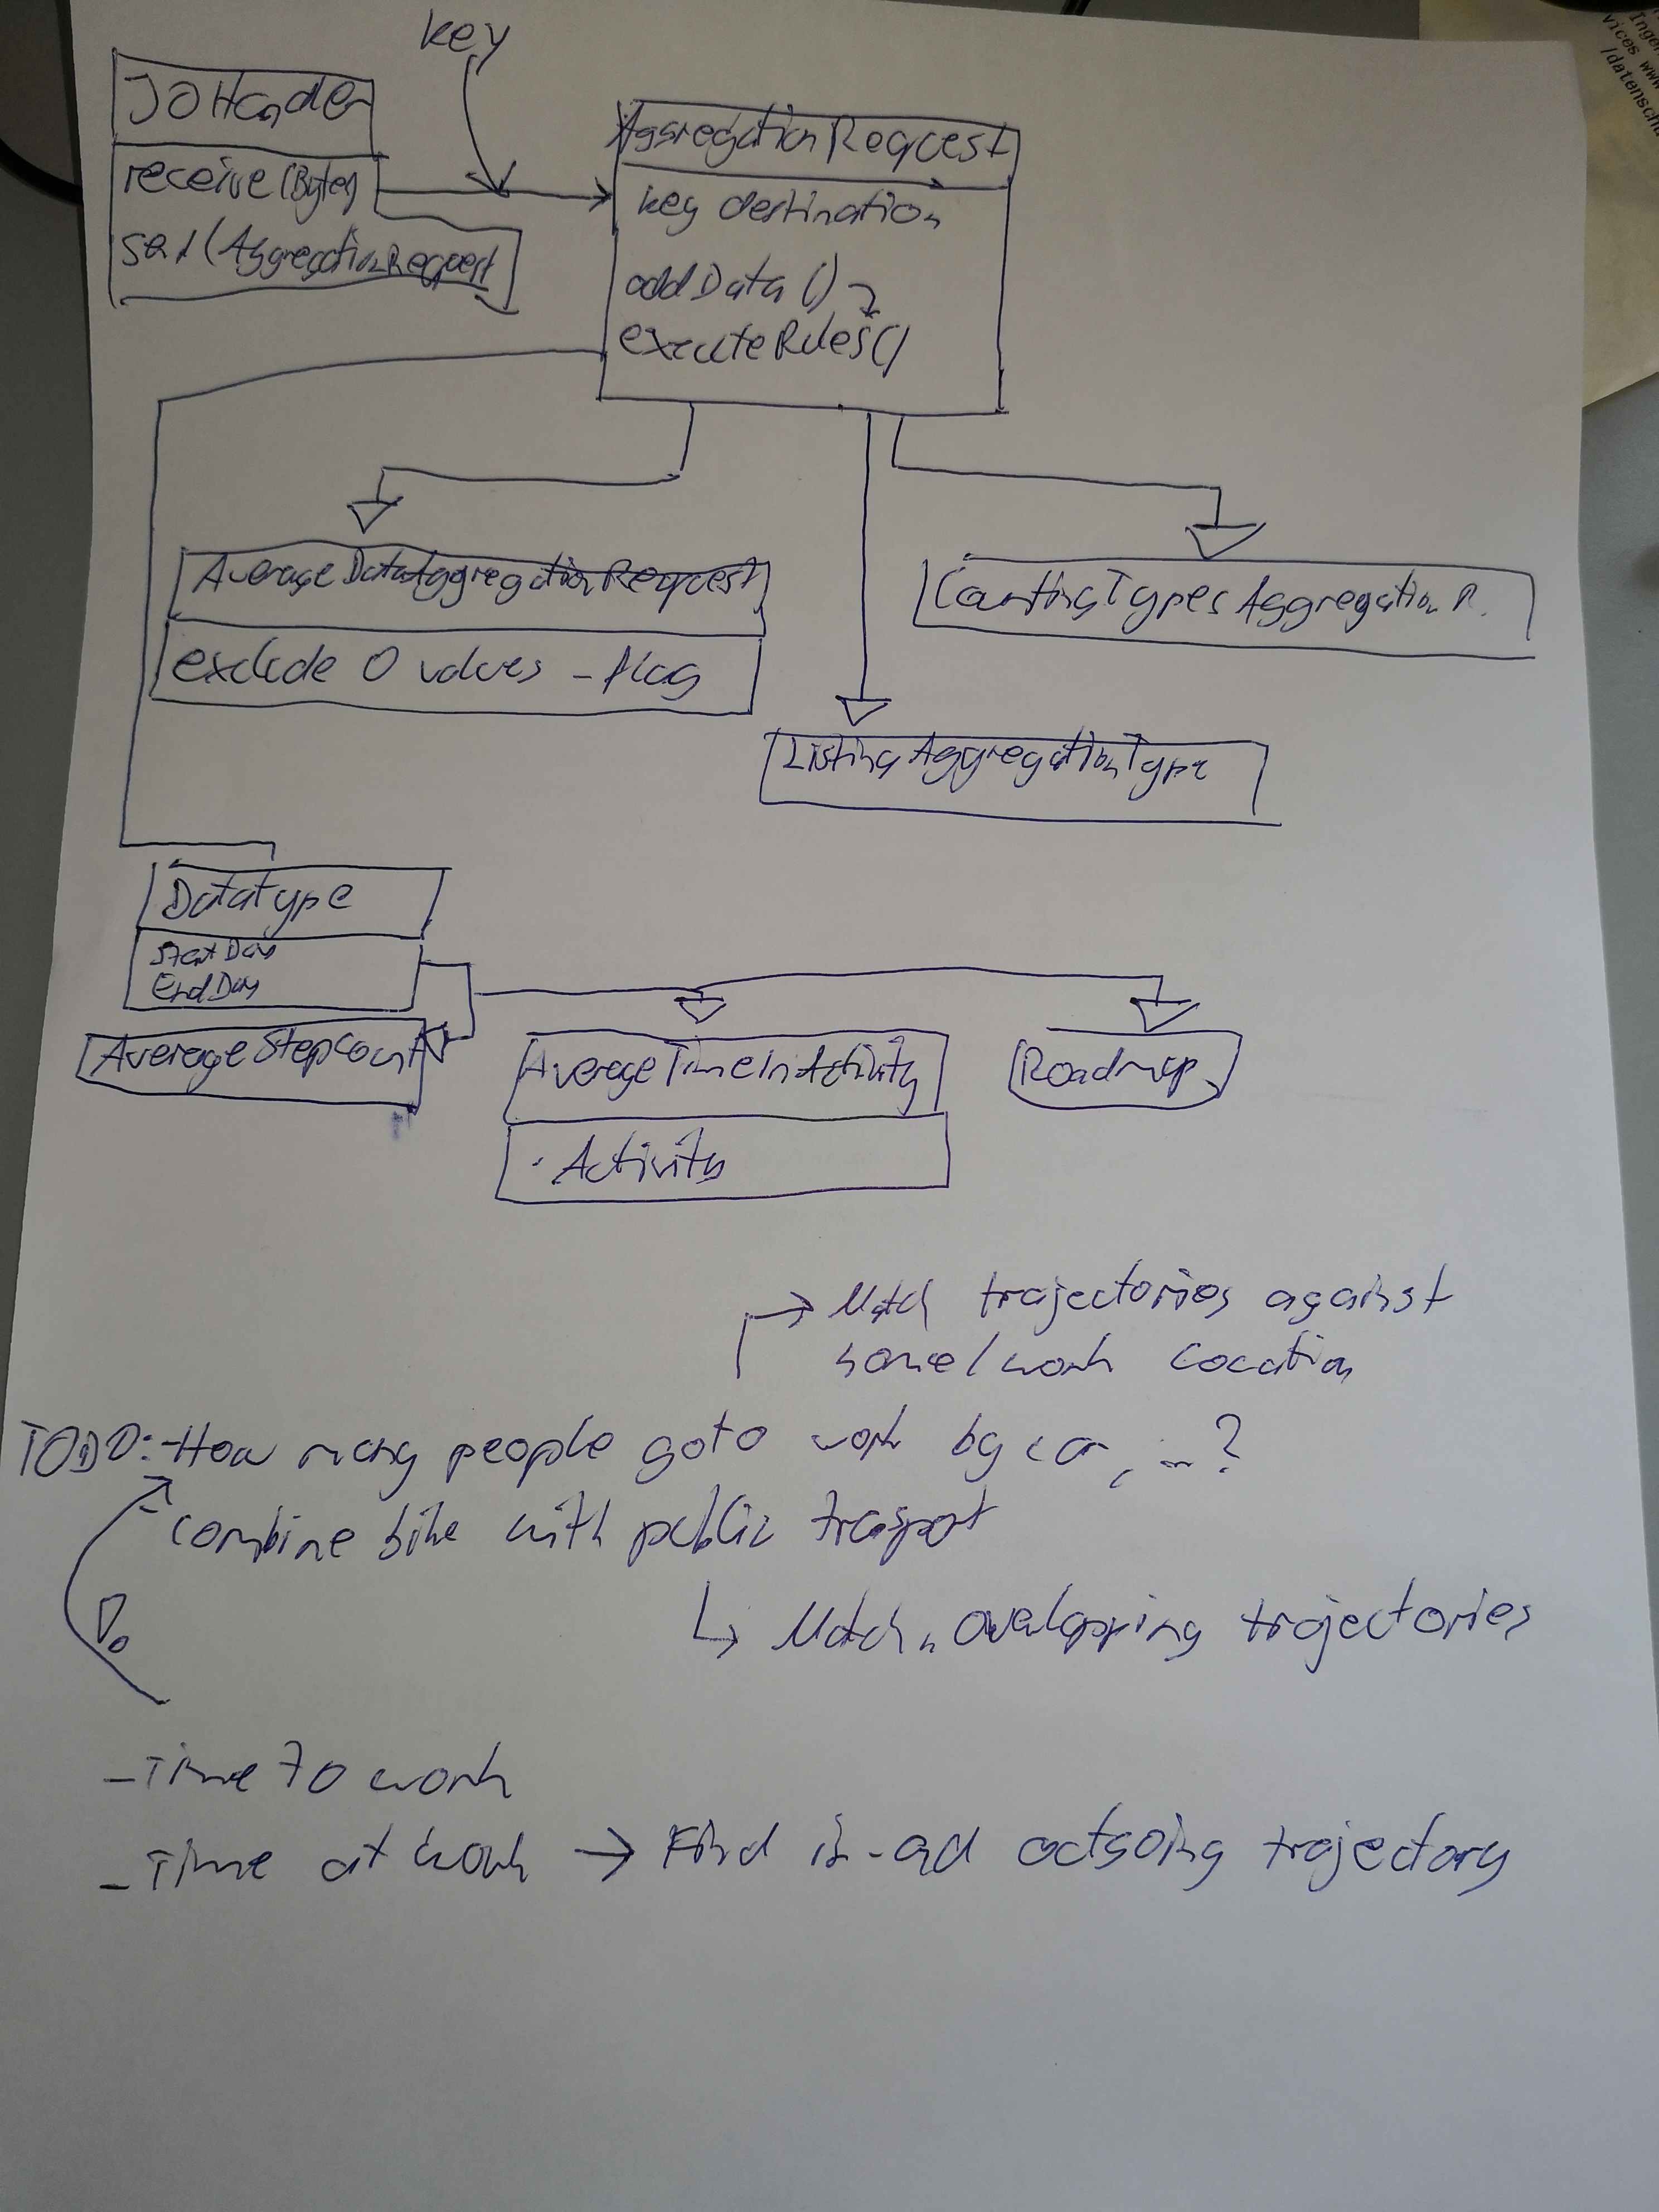
\includegraphics[width=\textwidth]{data/class-diagram-data-aggregation-requests.jpg}

\subsubsection{\textcolor{green}{Average step count}}
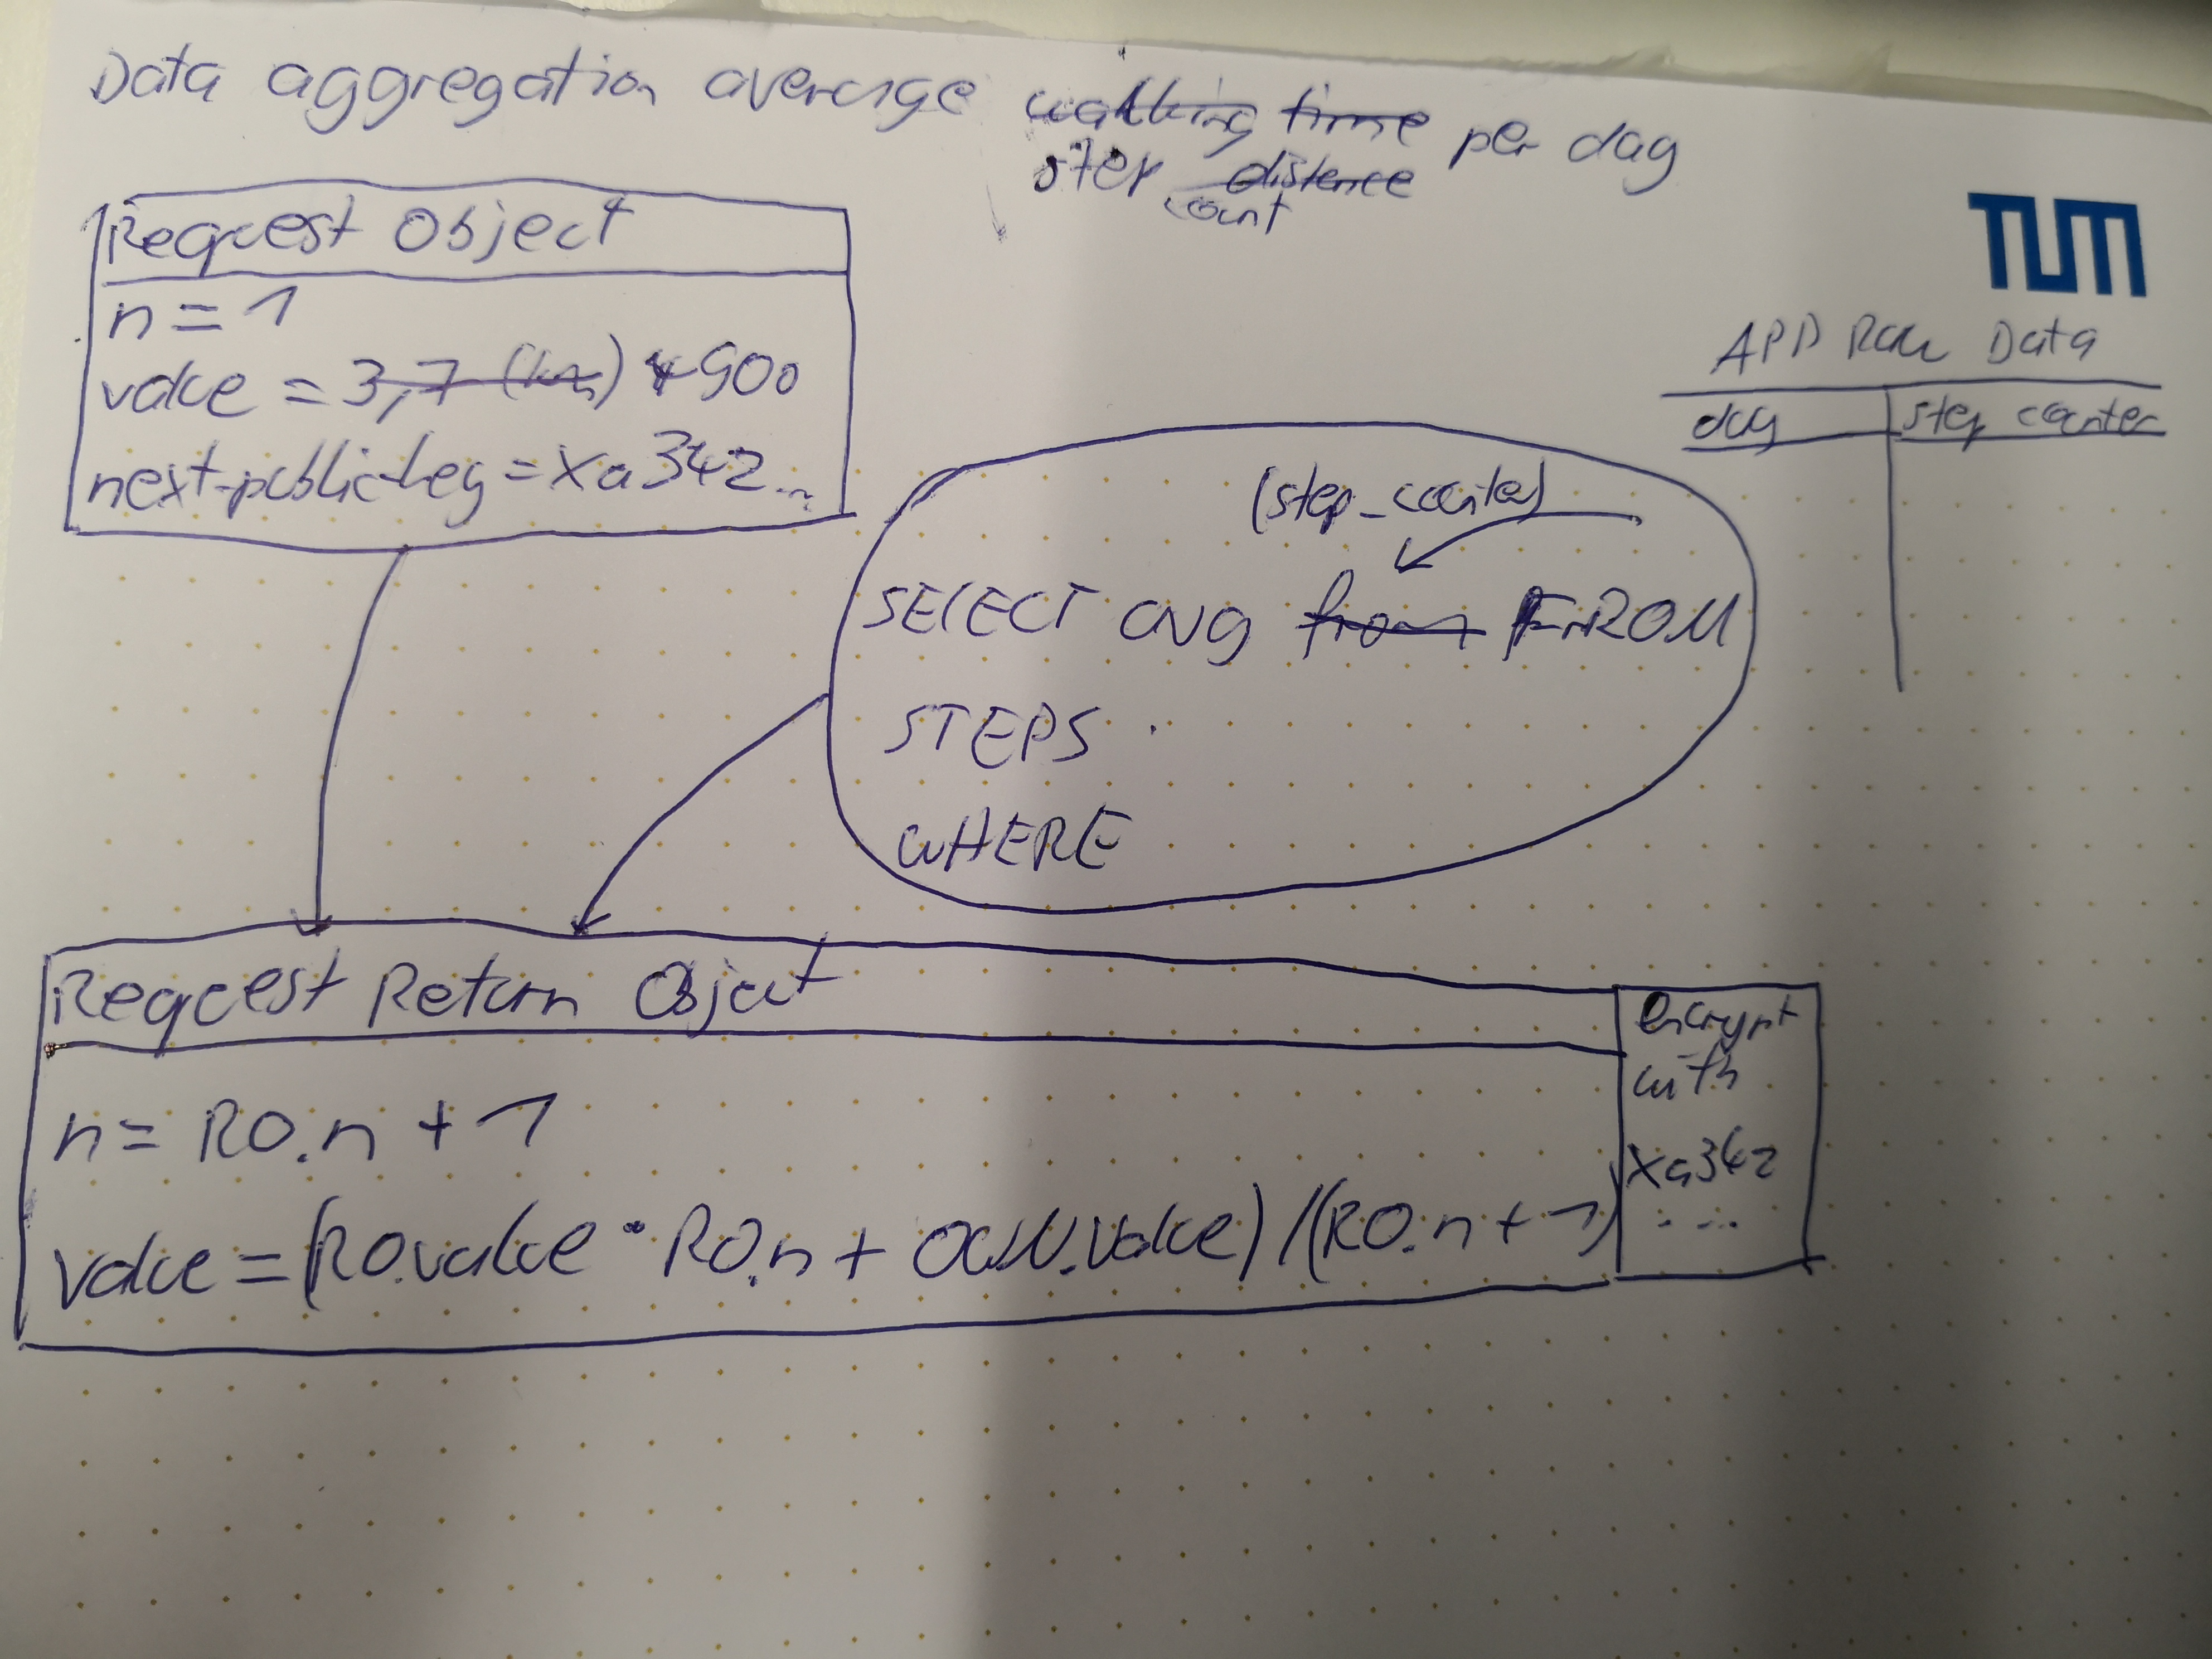
\includegraphics[width=\textwidth]{data/data-aggregation-average-step.jpg}

\subsubsection{\textcolor{green}{Average walking, driving, ... time}}
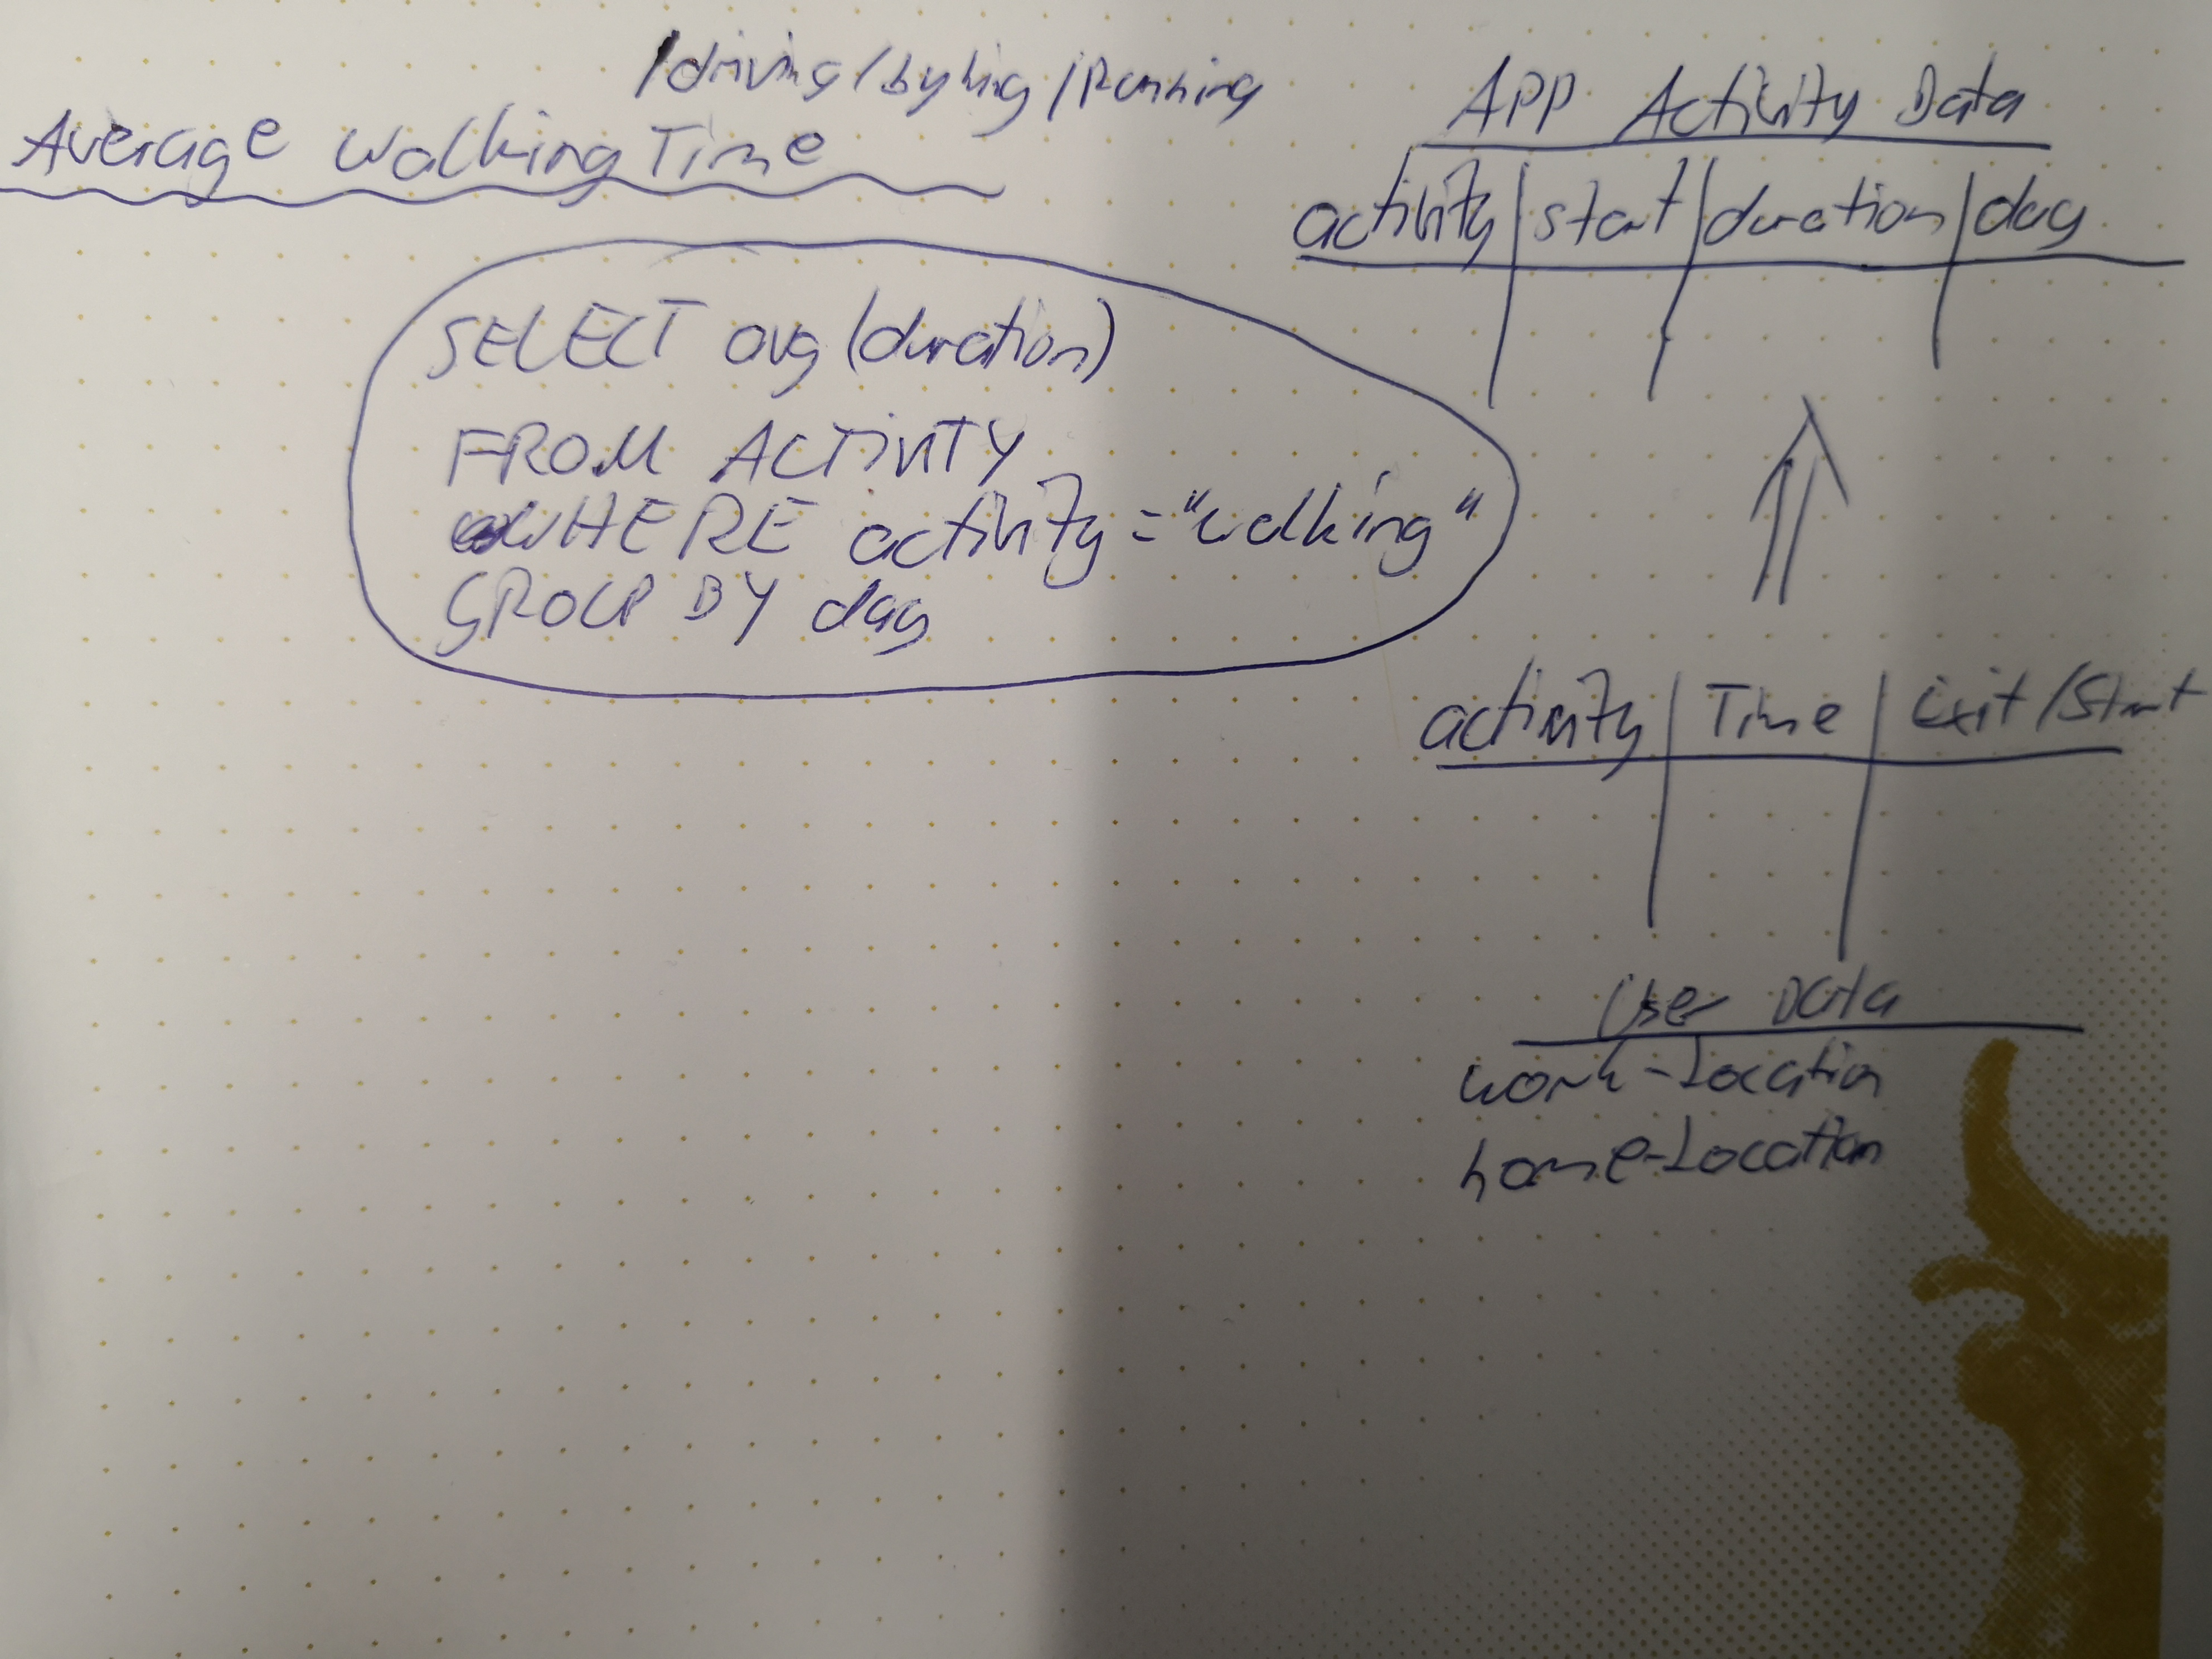
\includegraphics[width=\textwidth]{data/data-aggregation-average-walking.jpg}
For each of the activities [walking, biking, driving a car, driving public transport] a request is emitted to compute average data.
The request can further for each activity exclude or include 0-value-computation. Other solution: the 0-values are counted and the average / median of the other data (only in case).

\subsubsection{\textcolor{green}{How many people go to work by car, ...}}
Search trajectory database for trajectories starting at the home location and ending at the work location and infer activity from other sensor data.
If there are trajectories matching home and work location, each trajectory is treated as a car trajectory, if there was only car and walk activities within the trajectory.
As bike trajectory, if there was only bike and walk activities and walk if there was only walk.
Each trajectory home-> work or work-> home is treated as one entry for counting. If none of the former matches, the trajectory is counted as not\_clear.
Need sophisticated methods to determine work time, ... 
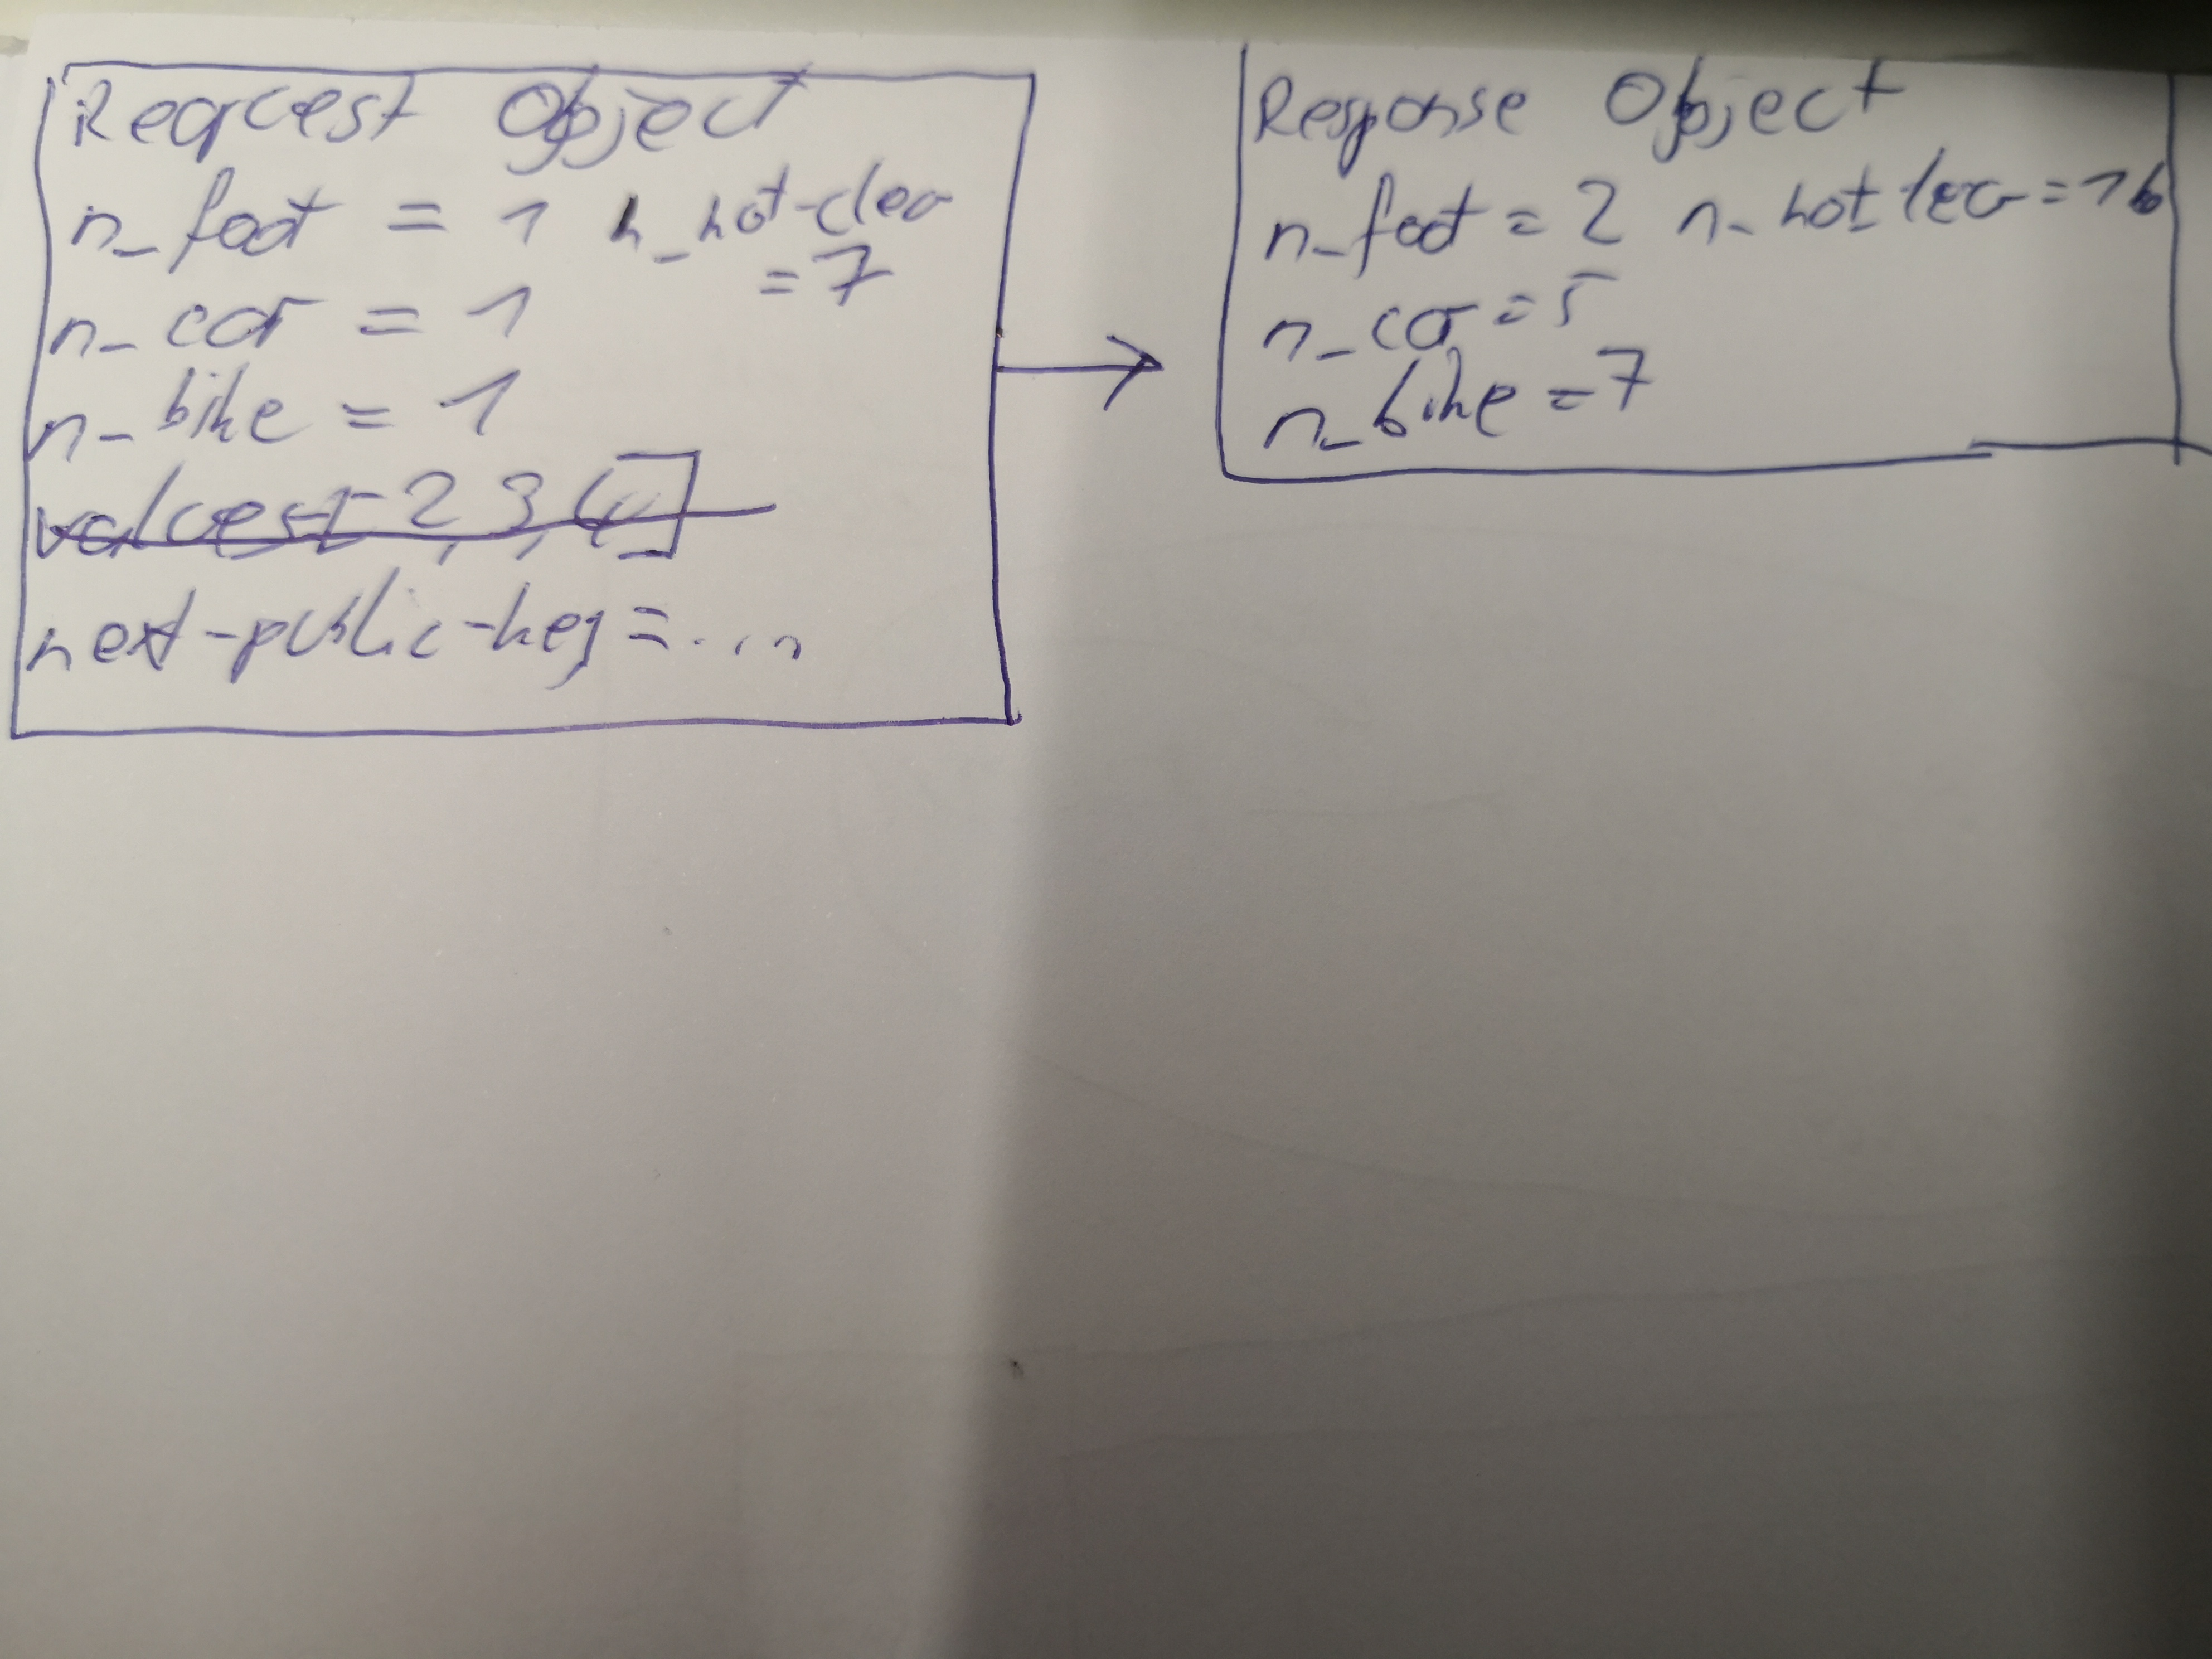
\includegraphics[width=\textwidth]{data/data-aggregation-transport-work-home.jpg}

\subsubsection{\textcolor{green}{How many people combine bike with public transport}}
select everybody where activity biking and activity public transport are close to each other.
As we cannot map public transport, we will use the driving activity in general.

\subsubsection{\textcolor{green}{Create a road map}}
The Request Object consists of a list of 2 location pairs associated with an activity. Only pairs with a spatial difference of less than XX meters are taken into account.
Aggregate all trajectories of the users longer than xx meter, cap the ends and the start for 50 meter, put similar trajectory coordinates together and publish the whole map.
A users data is only included, if in a radius of xx there are xx more --> k-anonymity.
Create a car / bike / walking map or color-code the map.

\subsubsection{\textcolor{green}{Compute the average speed (taking daytime into account) for roads}}
Filter for gps points that happen during driving or biking. Determine the speed 1. by the speed sensor measurement and 2. by the subsequent gps points.
This can e.g. be used to identify roads where zone 30 will reduce noise and co2 exhaustion a lot, if one can compute, that cars accelerate and then typically rest again, so that an average of 30 would have the same timing result. [TODO: Cite cities, ... where 30 is the limit in citycenter, ...]

\subsubsection{\textcolor{green}{Time to work}}
Compute, how much time on average a user needs to go to work.
This requires implementing locally the calculation of a users work and home place from the data (or we could also ask for the data and state that it will be locally only) or combine the two approaches.

\subsubsection{\textcolor{green}{Average time at work}}

\subsubsection{How much time do people usually spend searching for a parking spot}
Select activity driving while the trajectory circles around the same spot
\subsubsection{Identify roads, where (maybe even including the current traffic light sequence) one would be faster with a bike (thus average speed of 20, 22, ...)}
\subsubsection{Identify routes that are faster by bike than by car}



\subsubsection{Stage 2: When moving on a specific road, report bad traffic}
We will fake this in a way that when somebody is driving (recognized activity), we will randomly trigger the application to send an alert.
This way we do not have to implement downloading the standard speeds for a road map, recognizing a user being on this road and then checking for less than usual speed.

\subsection{Data Models}
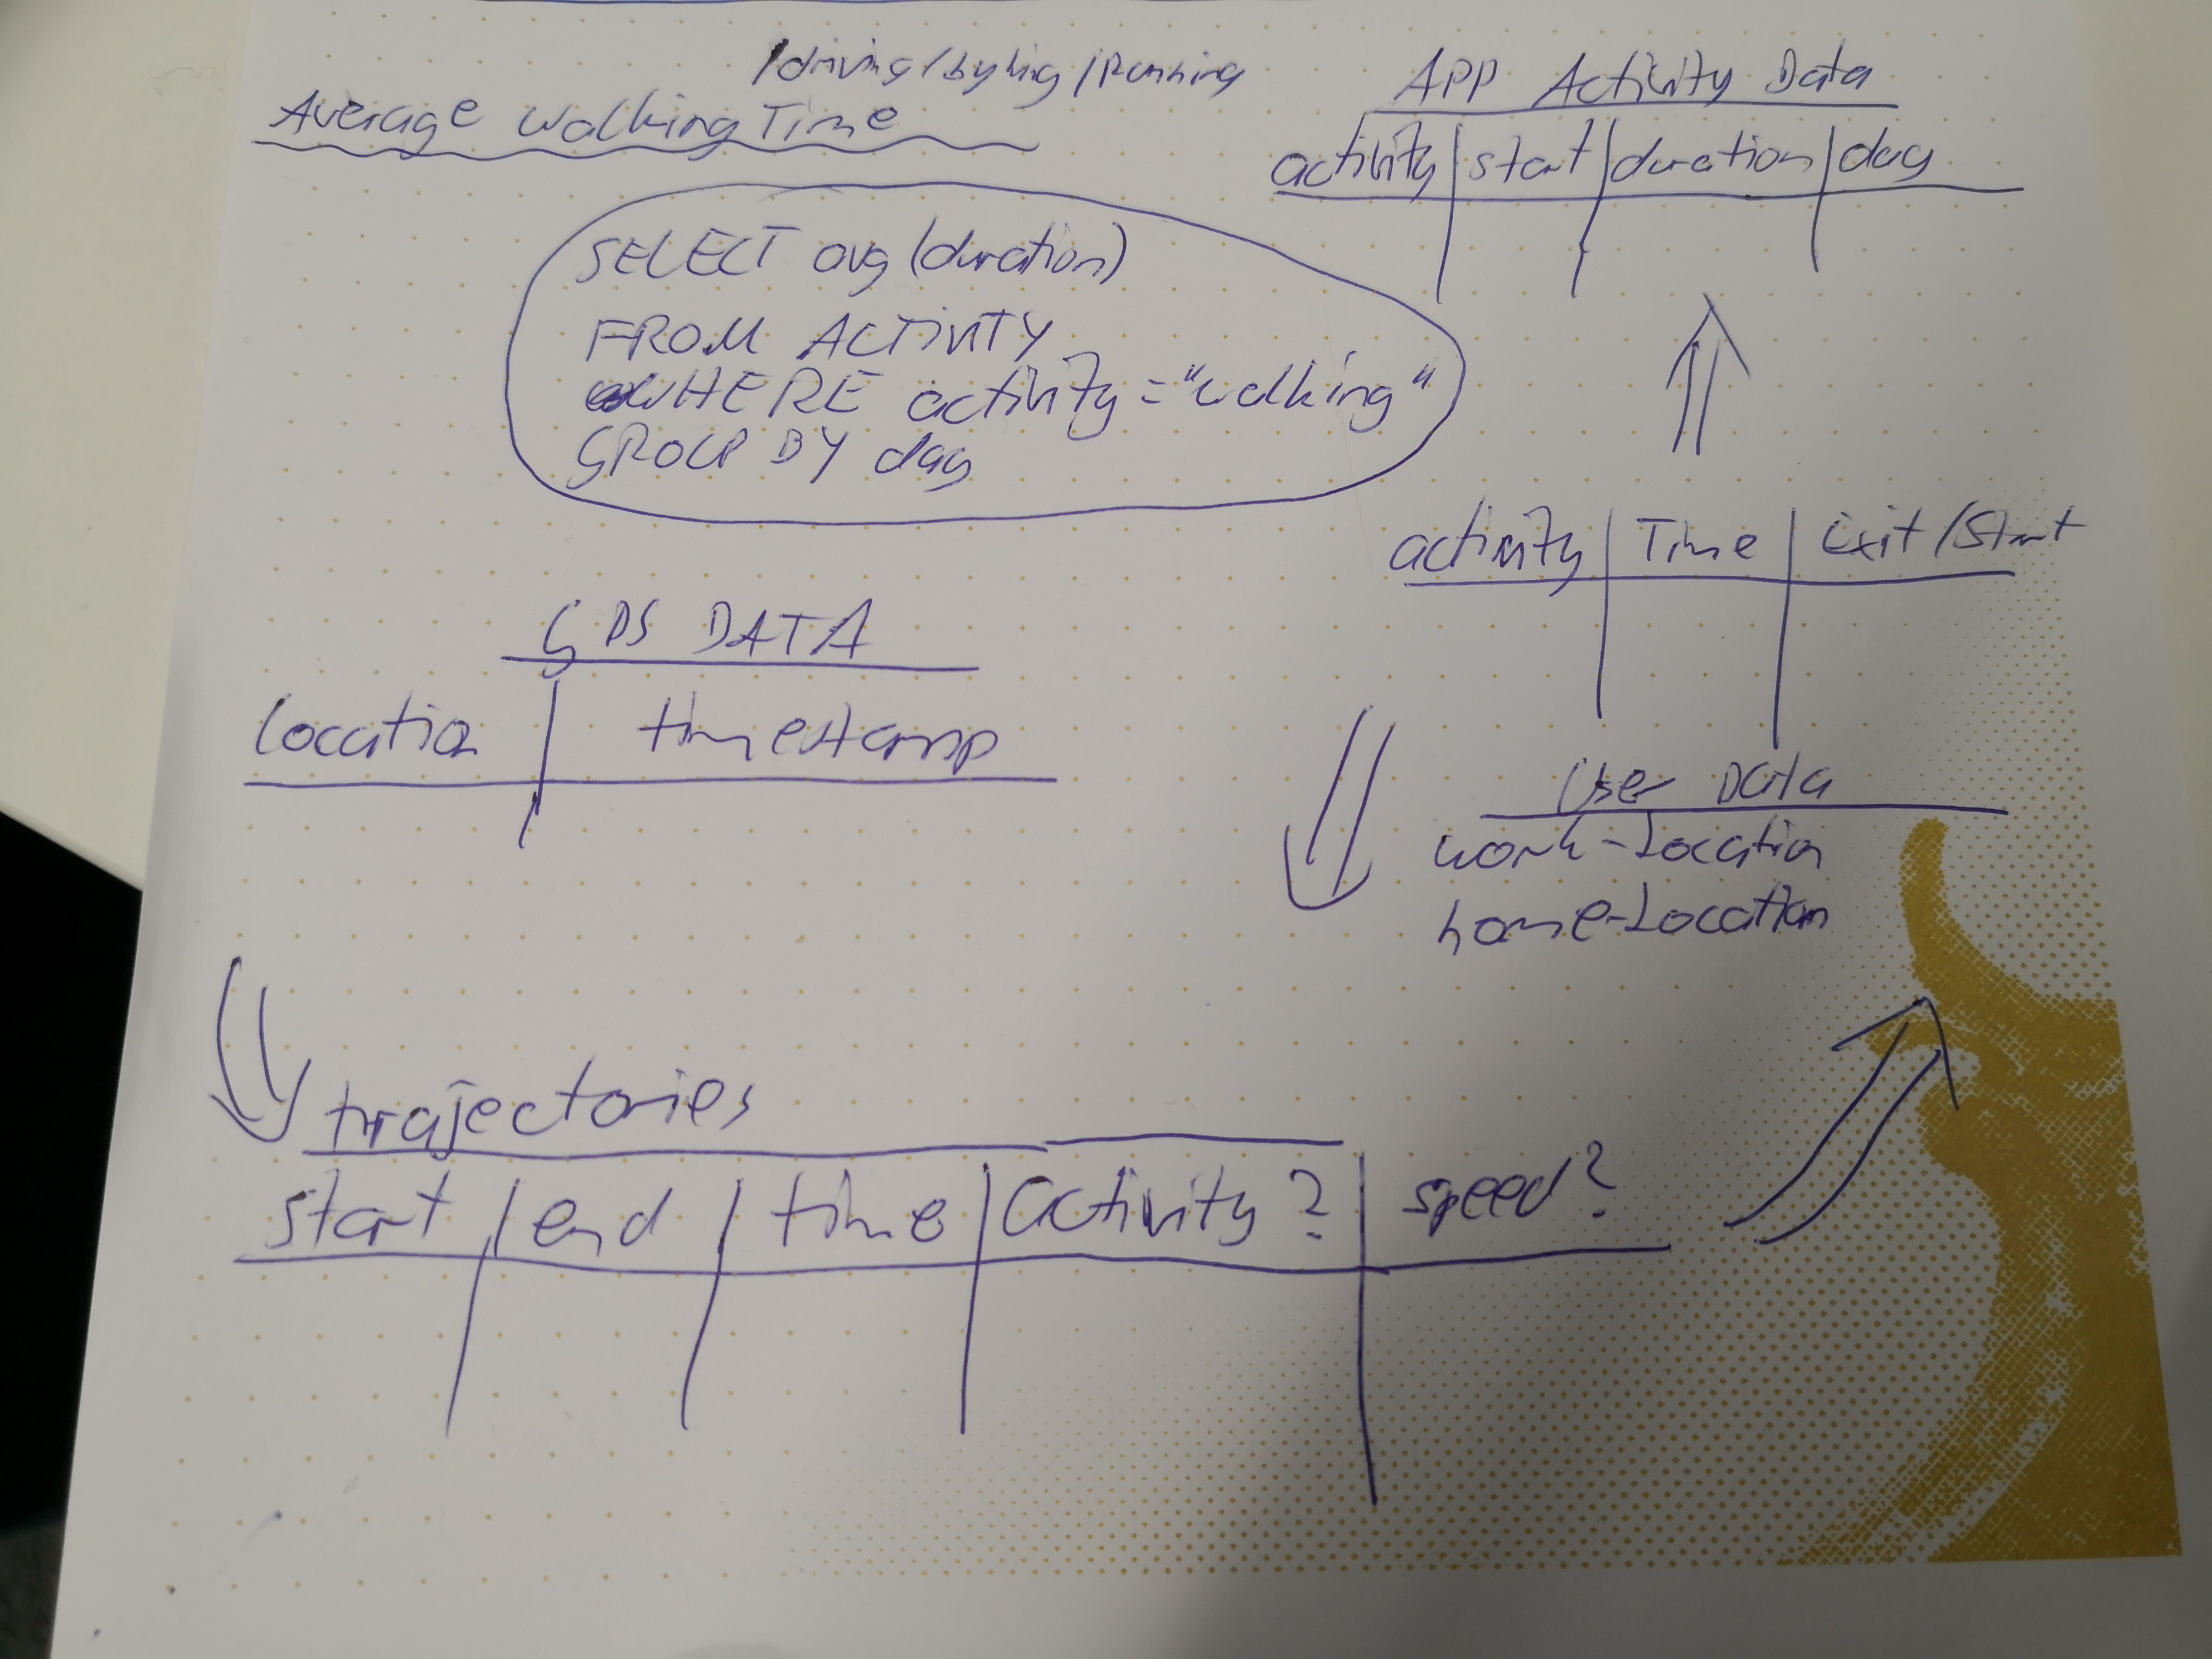
\includegraphics[width=\textwidth]{data/data-model.jpg}

\begin{itemize}
	\item \begin{verbatim}
	CREATE TABLE steps (
	day TEXT,
	steps INT
	);
	\end{verbatim}
	\item \begin{verbatim}
	CREATE TABLE activities (
	day TEXT,
	activity INT,
	start TEXT,
	duration INT,
	FOREIGN KEY (activity) REFERENCES activity_type (id)
	);
	\end{verbatim}
	\item \begin{verbatim}
	CREATE TABLE location (
	longitude REAL,
	lattitude REAL,
	speed REAL
	);
	\end{verbatim}
	\item \begin{verbatim}
	CREATE TABLE gps_data (
	location INT
	timestamp TEXT,
	FOREIGN KEY (location) REFERENCES location (id)
	);
	\end{verbatim}
	\item \begin{verbatim}
	CREATE TABLE trajectories (
	start INT,
	end INT,
	time_start TEXT,
	time_end TEXT,
	activity INT,
	FOREIGN KEY (activity) REFERENCES activity_type(id)
	FOREIGN KEY (start) REFERENCES location (id)
	FOREIGN KEY (end) REFERENCES location (id)
	);
	\end{verbatim}
\end{itemize}

\section{Implementation}
\subsection{Android Application}
We will base our implementation on \cite{gpsLogger}. [TODO: quit battery efficient] They provide the open-source code of an application logging a devices location at regular intervals to a file. We will adapt the logging to use json format and adhere to the standards of schema.org. We will furhter use reverse-geo-coding to determine the postal-code, city, region and country of GPS coordinates. The format used will adhere to the standard of \cite{schemaOrg}. For reverse-geo-coding we will use the google-api: \cite{googleApiReverseGeo}. The rsa public private key encryption will follow the example of \cite{rsa}. The raw data on the mobile device will either be stored using sqLite or using googles room: %https://developer.android.com/training/data-storage/room. https://bitbucket.org/tiitha/backgroundserviceexample/src/605ab7c73352ce57dfdde32d9e8ac97dfb661daf/app/src/main/java/com/geoape/backgroundlocationexample/BackgroundService.java?at=master&fileviewer=file-view-default Provides an example of how to let an applicataion run in the background.